\documentclass[11pt]{beamer}

%%%%%%%% tema e cor %%%%%%%%
\mode<presentation> {
\usetheme{Madrid}
%\usecolortheme{albatross}
}

\usepackage[utf8]{inputenc}
\usepackage{graphicx} 
\usepackage{booktabs}
\usepackage{subcaption}


\institute[HU-Berlin] 
{
\includegraphics[width=1.8cm]{img/logo-hu.png}
}

%%%%%%%% titulo e subtitulo %%%%%%%%
\title[Maximum Cardinality Matching]{Maximum Cardinality Matching Problem} 

%%%%%%%% nome dos autores %%%%%%%%
\author [Bojikian, Witkowski, Vogel]{Narek Bojikian, Piotr Witkowski, Martin Vogel} 

\begin{document}

\begin{frame}
\titlepage 
\end{frame}

%%%%%%%% slides %%%%%%%%
\section{Introduction} 
\begin{frame}{Assignment Problem}
\begin{figure}
    \centering
    \includegraphics[height=5cm]{img/introduction/assignment.png}
\end{figure}
\end{frame}

\begin{frame}{Definitions}
    \begin{itemize}[<+->]
    \item Matching
    \item \textbf{Perfect} Matching
    \item \textbf{Bipartite} Matching
    \item \textbf{Maximum} Matching
    \end{itemize}
  
  %add different figure for perfect matching and bipartite matching  
\only<1>{
	\begin{figure}
	\begin{subfigure}{.5\textwidth}
	\centering
	\includegraphics[width=.4\linewidth]{img/introduction/graph01.eps}	
	\end{subfigure}%
	\begin{subfigure}{.5\textwidth}
	\centering
	\includegraphics[width=.4\linewidth]{img/introduction/graph02.eps}
	\end{subfigure}
	\end{figure}
}
\only<2>{
	\begin{figure}
	    \centering
	    \includegraphics[width=0.3\linewidth]{img/introduction/perfectmatching.eps}
	\end{figure}
}
\only<3>{
	\begin{figure}
	\begin{subfigure}{.5\textwidth}
	\centering
	\includegraphics[width=.4\linewidth]{img/introduction/bipar.eps}
	\end{subfigure}%
	\begin{subfigure}{.5\textwidth}
	\centering
	\includegraphics[width=.4\linewidth]{img/introduction/biparmatch.eps}
	\end{subfigure}
	\end{figure}
}
\only<4>{
	\begin{figure}
	\begin{subfigure}{.5\textwidth}
	\centering
	\includegraphics[width=.4\linewidth]{img/introduction/maximalmatch.eps}
	\end{subfigure}%
	\begin{subfigure}{.5\textwidth}
	\centering
	
\includegraphics[width=.4\linewidth]{img/introduction/maximummatching.eps}
	\end{subfigure}
	\end{figure}
}
    
\begin{block}{Definition}
    \only<1>{A set of non overlapping edges.}
    \only<2>{Matching of size $\frac{|V\left(G\right)|}{2}$}
    \only<3>{Matching on a bipartite graph.}
    \only<4>{Matching of the maximum size.}
\end{block} 
\end{frame}

\begin{frame}{Maximum Matching vs Maximal Matching}
	\parbox[c][.7\textheight][c]{\textwidth}{%
		\only<1>{
			\begin{center}
				\includegraphics[width=0.15\linewidth]{img/random/maximum-maximal-0.eps}
			\end{center}
		}
		\only<2>{
			\begin{center}
				\includegraphics[width=0.15\linewidth]{img/random/maximum-maximal-1.eps}
			\end{center}
		}
		\only<3->{
			\begin{center}
				\includegraphics[width=0.15\linewidth]{img/random/maximum-maximal-2.eps}
			\end{center}
		}
		\uncover<4>{
			\begin{center}
				\includegraphics[width=0.15\linewidth]{img/random/maximum-maximal-3.eps}
			\end{center}
		}
	}
\end{frame}


\section{Matching algorithms} 
\begin{frame}{Hall's Theorem}
\only<1>{
\begin{figure}
\end{figure}
}
\begin{block}{Definition}
    \only<1>{A bipartite graph G consisting of sets U and W, has a matching satisfying $|u|$ if and only if $|N(x)| \geq |x|$ for every nonempty subset X of U.}
\end{block} 
\end{frame}

\begin{frame}{Examples - Hall's Theorem}
- Examples on the board --

\end{frame}
  
\begin{frame}{Königs Theorem}
\only<1>{
\begin{figure}
\end{figure}
}
\begin{block}{Definition}
    \only<1>{The maximum matching for a bipartite graph equals its minimum vertex cover}
\end{block} 
\end{frame}

\begin{frame}{Königs Theorem - Example}
-- Example on the Board -- 
  
\end{frame}

\begin{frame}{Alternating Path}
\centering
\includegraphics[width=.4\linewidth]{img/bipartite/alternating1.png}
\only<1>{
\begin{figure}
\end{figure}
}
\begin{block}{Definition}
    \only<1>{Let $G = (X, Y, E)$ be a bi-partite graph where the vertices are divided into the sets X and Y and E the edges.}
\end{block} 
\end{frame}

\begin{frame}{Alternating Path}
\includegraphics[width=.8
\linewidth]{img/bipartite/alternating2.png}
  
\end{frame}

\begin{frame}{Alternating Path}
\includegraphics[width=.8\linewidth]{img/bipartite/alternating3.png}
  
\end{frame}

\begin{frame}{Alternating Path - Summary}
- starts in a vertex element of X and ends in vertex element of Y\newline
- must have an odd-number of edges\newline
- will visit nodes in X und Y alternatedly\newline
- And it starts and ends in free/unmatched vertices\newline
\newline
$\rightarrow$ To go forward, use an edge that is not part of the matching\newline
$\rightarrow$ To go backward, use an edge that is part of the matching\newline
  
\end{frame}

\begin{frame}{Augmenting Path - Definition}
\only<1>{
\begin{figure}
\end{figure}
}
\begin{block}{Definition}
    \only<1>{An augmenting path is an alternating path where the first and last vertex are unmatched.}
\end{block} 
\end{frame}

\begin{frame}{Augmenting Path - example}
-- Example on the Board --
  
\end{frame}

\begin{frame}{Breadth First Search - repetition}
-- Example on the Board --
  
\end{frame}

\begin{frame}{Berge Theorem}
A matching is a maximum matching if it contains no augmenting path.
  
\end{frame}

\begin{frame}{Hungarian Method}
Search augmenting paths in the graph until no augmenting path can be found\newline
\newline
$\rightarrow$ \textbf {Time complexity: $O(|V|^3)$}\newline
\newline
Precise information can be found here: \textbf {https://brilliant.org/wiki/hungarian-matching/}\newline
\newline
\textbf {Note}: It is not an algorithm, so it does not specify a implementation
\end{frame}

\begin{frame}{Maximum Flow Reduction}
-- Example on the Board --
  
\end{frame}

\begin{frame}{Hopcraft-Carp Algorithm}
Input: \textbf{A bipartite Graph}
Initialize Matching\newline
1. Repeat\newline
$\rightarrow$ Build alternating level graph rooted at unmatched vertices using bfs\newline
$\rightarrow$ Augment M via maximal set of vertex disjoint shortest-length paths\newline
$\rightarrow$ until no augmenting paths exists\newline
2. Return M\newline
		
\textbf {Time complexity: $O(|E|*\sqrt{|V|})$}
  
\end{frame}

\begin{frame}{Hopcraft-Carp Algorithm - bipartite Graph}

-- Example on the Board --
  
\end{frame}

\begin{frame}{}
	\centering \textbf{\huge General graphs}
\end{frame}

\begin{frame}[t]{General graphs}
	\textbf{Problem:} odd-length cycles\\
	%images with 6 edges, 5 edges in a cycle and one more adjacent edge
	
	\begin{center}
	Maximal: matching of size 2
	\includegraphics[width=0.35\linewidth]{img/general/odd-matching-maximal.eps}
	\end{center}

	\begin{center}
	Optimum: matching of size 3
	\includegraphics[width=0.35\linewidth]{img/general/odd-matching-optimal.eps}
	\end{center}
\end{frame}

\begin{frame}[t]{General graphs}
	Bipartite graphs can have cycles, but always only of even length:\\
	
	\begin{center}
	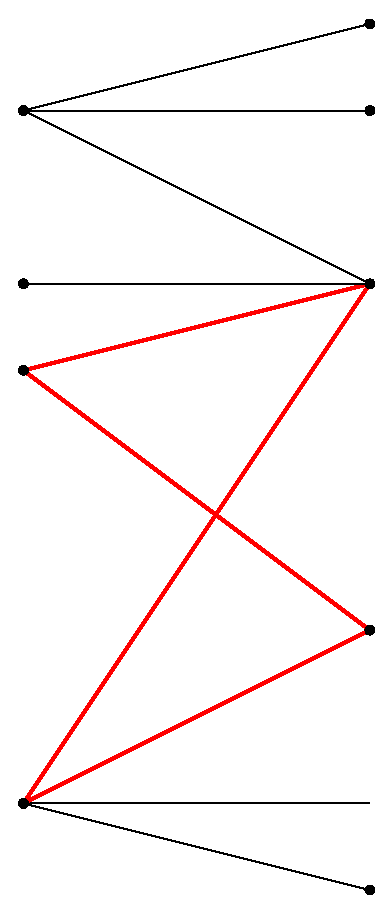
\includegraphics[width=0.2\linewidth]{img/general/bipartite-even-cycle.eps}	
	\end{center}	
\end{frame}

\begin{frame}[t]{Edmonds' Blossom algorithm (1961)}
	\only<1->{Blossom algorithm uses the idea of Berge's Theorem, that}
	
	\only<2->{matching is a \textbf{maximum matching} iff there is \textbf{no augmenting path}.}
	
	\only<3->{
		\vspace{1em}
		\textbf{Input:} Graph $\mathcal{G}$, initial matching $\mathcal{M}$ on $\mathcal{G}$\\
		\textbf{Output:} maximum matching $\mathcal{M^*}$ on $\mathcal{G}$	
	}

	\only<4->{
		\vspace{1em}
		In other words, Blossom algorithm improves existing matching $\mathcal{M}$ in $\mathcal{G}$ as long as augmenting paths exist, then returns.	
	}
\end{frame}

\begin{frame}[t]{Edmonds' Blossom algorithm (1961)}
	\begin{center}
	\includegraphics[width=0.8\linewidth]{img/general/Edmonds_augmenting_path.png}
	\end{center}
\end{frame}

\begin{frame}[t]{Edmonds' Blossom algorithm (1961)}
	\only<1->{
		\textbf{Problem:} How to guarantee no augmenting paths in a graph?
	}

	\only<2->{
		\vspace{1em}
		\textbf{Schema:} 
		\begin{itemize}
			\item shrink the graph in a way, that preserves augmenting paths
			\item extend matching when possible
			\item return, when no augmenting path found
		\end{itemize}
	}
\end{frame}

\begin{frame}[t]{Edmonds' Blossom algorithm (1961)}
	\textbf{Example:}
	
	[TODO: include images]
\end{frame}

\begin{frame}[t]{Edmonds' Blossom algorithm (1961)}
	\textbf{Pseudocode:}\\
	[TODO: include pseudocode]
	
	\vspace{1em}
	\textbf{Complexity:} [TODO: include complexity]

\end{frame}

\section{Randomized Algorithm for matching} 
\begin{frame}{}
	\centering \textbf{\huge A short review..}
\end{frame}

\begin{frame}{Maximum Matching vs Maximal Matching}
	\parbox[c][.7\textheight][c]{\textwidth}{%
\only<1>
{
	\begin{center}
    \includegraphics[width=0.15\linewidth]{img/random/maximum-maximal-0.eps}
	\end{center}
}
\only<2>
{
	\begin{center}
    \includegraphics[width=0.15\linewidth]{img/random/maximum-maximal-1.eps}
	\end{center}
}
\only<3->
{
	\begin{center}
    \includegraphics[width=0.15\linewidth]{img/random/maximum-maximal-2.eps}
	\end{center}
}
\uncover<4>
{
	\begin{center}
    \includegraphics[width=0.15\linewidth]{img/random/maximum-maximal-3.eps}
	\end{center}
}
}
\end{frame}

\begin{frame}[t]{Determinant and Permanent}
	A short trip in mathematics,\\
	\textbf{Permutation} - Bijection over $n$ elements.\\
	$\mathcal{S}_n$ - Set of all permutatoins of $n$ elements.\\~\\
	For an $n\times n$-matrix $A$, we define

\begin{columns}[T] % align columns\end{column}%
\begin{column}{.48\textwidth}
	{\centering \textbf{Determinant of a matrix}\\}
$$det(A) =  \sum\limits_{\pi \in \mathcal{S}} sign(\pi) \prod\limits_{i\in[n]} A_{i, \pi(i)}$$
	laplace expansion (on board).\\
	Efficient Gaussian Eliminatin.\\
	$O(n^\omega), \omega = 2.373$.\\
	Matrix-Multiplication Exponent.\\

\end{column}
\hfill%
\begin{column}{.48\textwidth}
	{\centering \textbf{Permanent of a matrix}\\}
$$perm(A) =  \sum\limits_{\pi \in \mathcal{S}}  \prod\limits_{i\in[n]} A_{i, \pi(i)}$$
	\textbf{NP-Hard} problem.\\
	Presumably no polynomial time algorithm to compute.\\

\end{column}
\end{columns}
\end{frame}

\begin{frame}[t]{Randomized Perfect Matching}
	How to check if a bipartite graph admits a perfect matching?\\

\begin{tabular}{cl}  
\begin{tabular}{c}
\only<1-2>
{
    \includegraphics[width=0.15\linewidth]{img/random/randombip-orig.eps}
}
\only<3->
{
    \includegraphics[width=0.15\linewidth]{img/random/randombip-matched.eps}
}
\end{tabular}
& \begin{tabular}{l}
\parbox{0.7\linewidth}{%  change the parbox width as appropiate
	\only<2-3>
	{
	\[
	A^G=
	\begin{bmatrix}
	1 & 1 & 0 \\
	0 & 1 & 1 \\
	1 & 0 & 0 
	\end{bmatrix}
	\]
	}
	\only<4->
	{
	\[
	A^G=
	\begin{bmatrix}
	1 & \textcolor{red}{1} & 0 \\
	0 & 1 & \textcolor{red}{1} \\
	\textcolor{red}{1} & 0 & 0 
	\end{bmatrix}
	\]
	}

\uncover<5->
{
	\begin{center}
	\begin{tabular}{|l|*{3}{c}|r}
		\hline
		$u_i$ & 1 &  2 & 3  \\
		\hline
		$\pi(u_i)$ & 2 &  3 & 1  \\
		\hline
	\end{tabular}
	\end{center}
}
}
\\
\end{tabular}
\end{tabular}
\only<6->
{
	The graph admits a perfect matching $\iff$\\
}
\only<7->
{
	There is a permutation $\pi$, s.t. $\prod\limits_{i \in [n]}A^G_{i, \pi(i)} = 1$  $\iff$\\
}
\only<8>
{
	For $\mathcal{S}$ the set of all permutations on $n$ elements
\[
	\sum\limits_{\pi \in \mathcal{S} } \prod\limits_{i \in [n]} A^G_{i, \pi(i)} > 0
\]
}
\only<9->
{
For $\mathcal{S}$ the set of all permutations on $n$ elements
\[
	\underbrace{\sum\limits_{\pi \in \mathcal{S} } \prod\limits_{i \in [n]} A^G_{i, \pi(i)}}_{perm(A^G)} > 0
\]
}
\end{frame}

\begin{frame}[t]{Permanent and Determinant}
	\begin{align*}
		perm(A) = & \sum\limits_{\pi \in \mathcal{S}} \prod\limits_{i\in[n]} A_{i, \pi(i)} & \uncover<2->{\dots\text{is a known hard problem}}\\
		\uncover<3->{det(A) = & \sum\limits_{\pi \in \mathcal{S}} sign(\pi) \prod\limits_{i\in[n]} A_{i, \pi(i)} & }
	\end{align*}

	\uncover<4->{We don't have to bound ourselves with ones in the matrix..\\}
	\uncover<5->{
	\begin{tabular}{cl}  
	\begin{tabular}{c}
    	\includegraphics[width=0.15\linewidth]{img/random/randombip-orig.eps}
	\end{tabular}
	\begin{tabular}{l}
	\parbox{0.7\linewidth}{%  change the parbox width as appropiate
	\[
	A'^G=
	\begin{bmatrix}
		x_{11} & x_{12} & 0 \\
		0 & x_{22} & x_{23} \\
		x_{31} & 0 & 0 
	\end{bmatrix}
	\]
	}
	\end{tabular}
	\end{tabular}
	}
	\uncover<6->{$det(A'^G)$ is a polynomial of degree $n$.\\}
	\uncover<7->{The graph admits a perfect matching $\iff$ the polynomial $det(A'^G)$ is not identical zero.}
\end{frame}

\begin{frame}[t]{Schwartz-Zippel lemma} 
	\begin{block}{Shwartz-Zippel lemma}
		Let $\rho$ be a non-zero polynomial of $n$ variables and degree $d$ over a field $\mathbb{F}$.\\
		Let $\mathcal{S} \subseteq \mathbb{F}^n$, then for $x_0 \underset{u.a.r}{\in} \mathcal{S}$
		$$Pr[\rho(x_0) = 0] \leq \frac{d}{|\mathcal{S}|}$$
	\end{block}
	\only<2->
	{
	Choosing $|\mathcal{S}| = 2d$, we get a method that tells with probability at least $1/2$, if the polynomial is identical zero.\\
	}
	\only<3->
	{
	Since one non-zero answer is enough to know the polynomial is a non-zero, we can repeat the operation a couple of times magnifying the probability.\\
	}
\end{frame}


\end{document}
